\documentclass[twocolumn]{article}
\usepackage[danish]{babel}
\usepackage[utf8]{inputenc}
\usepackage[T1]{fontenc}
\usepackage[margin=0.4in]{geometry}
\usepackage{graphicx}
\usepackage[font=small,labelfont=bf]{caption}
\setlength{\columnsep}{0.3in}
\title{Kilonovaen og oprindelsen af guld}
\author{Jonatan Selsing, The Cosmic Dawn Center, Niels Bohr Instituttet, Københavns Universitet}
%\date{\today}
\date{\vspace{-3ex}}

\begin{document}

\maketitle


\begin{abstract}
I denne her artikel vil jeg introducere et fænomen, som først for ganske nyligt er trådt frem på den astronomiske scene, nemlig kilonovaer. Kilonovaer har vist sig at være nogle af de mest eksotiske, sjældne og samtidig betydningsfulde begivenheder, der sker i universet. En kilonova er et resultat af sammenstødet mellem to neutronstjerner eller en neutronstjerne og et sort hul. I sammenstødet bliver neutronstjernemateriale slynget ud i universet, og dette materiale bliver til alle de tungeste grundstoffer vi kender, som bl.a. guld, sølv og platin. 
\end{abstract}

\section{Introduktion}
Den 17. august 2017 skete der noget specielt i de tre tyngdebølgedetektorer, der bliver drevet af det, der kaldes LIGO/Virgo-samarbejdet. For første gang registrerede detektorerne det karakteristiske "tyngdebølge-skvulp" fra et binært system, hvis totale vægt var mindre end ca. 2.8 solmasser, hvilket svarer til massen af to neutronstjerner \cite{abbotta}. Uafhængigt heraf, og forsinket med 1.7 s, detekterede GBM-instrumentet (Gamma-ray Burst Monitor) om bord på rum-teleskopet \textit{Fermi} et kort signal af gammastråler, der tilsvarer den type signal, vi kender fra såkaldte korte gammaglimt. Derfra vidste vi med det samme, at tyngdebølgesignalet rejste sammen en eller anden form for elektromagnetisk stråling. Det betød, at vi for første gang i verdenshistorien havde muligheden for at se det optiske modstykke til et tyngdebølge-signal. Dette optiske modstykke var på forhånd blevet anslået til at være lysstærkt nok til, at vi ville kunne se det, og samtidig havde teoretikere forudset, at det potentielt set kunne være kilden til alle de tungeste grundstoffer i universet \cite{lattimer}. På grund af formodningen om, at modstykket ville være betydningsfuldt, var det vigtigt at sikre en hurtig opfølgning med teleskoper, inden det optiske lys blev for svagt til at se. 

Ved at triangulere på baggrund af ankomsttidspunktet af signalet i tyndebølgedetektorerne kunne LIGO/Virgo finde frem til, at dette her sammenstød skete over den sydlige halvkugle inden for et område på størrelse med fuldmånen, hvilket er ca. 28 kvadratgrader. Dette lyder måske ikke af meget, men en typisk størrelse, som et teleskop dækker, er omkring 0.25 kvadratgrad, så det kræver alligevel en del billeder at dække hele området. 10.9 timer efter den simultane observation af tyngdebølger og gamma-stråler blev det optiske modstykke fundet. Detektions-billederne er vist i figur \ref{fig1}, hvor det øverste, højre billede er det første billede, der blev taget af kilonovaen. Så snart det optiske modstykke blev fundet, var den positionelle usikkerhed så lille, at en verdensomspændende opfølgningskampagne kunne iværksættes, hvor teleskoper, der dækker hele det elektromagnetiske spektrum, kunne pege mod dette nyopdagede astronomiske fænomen.

\begin{figure}
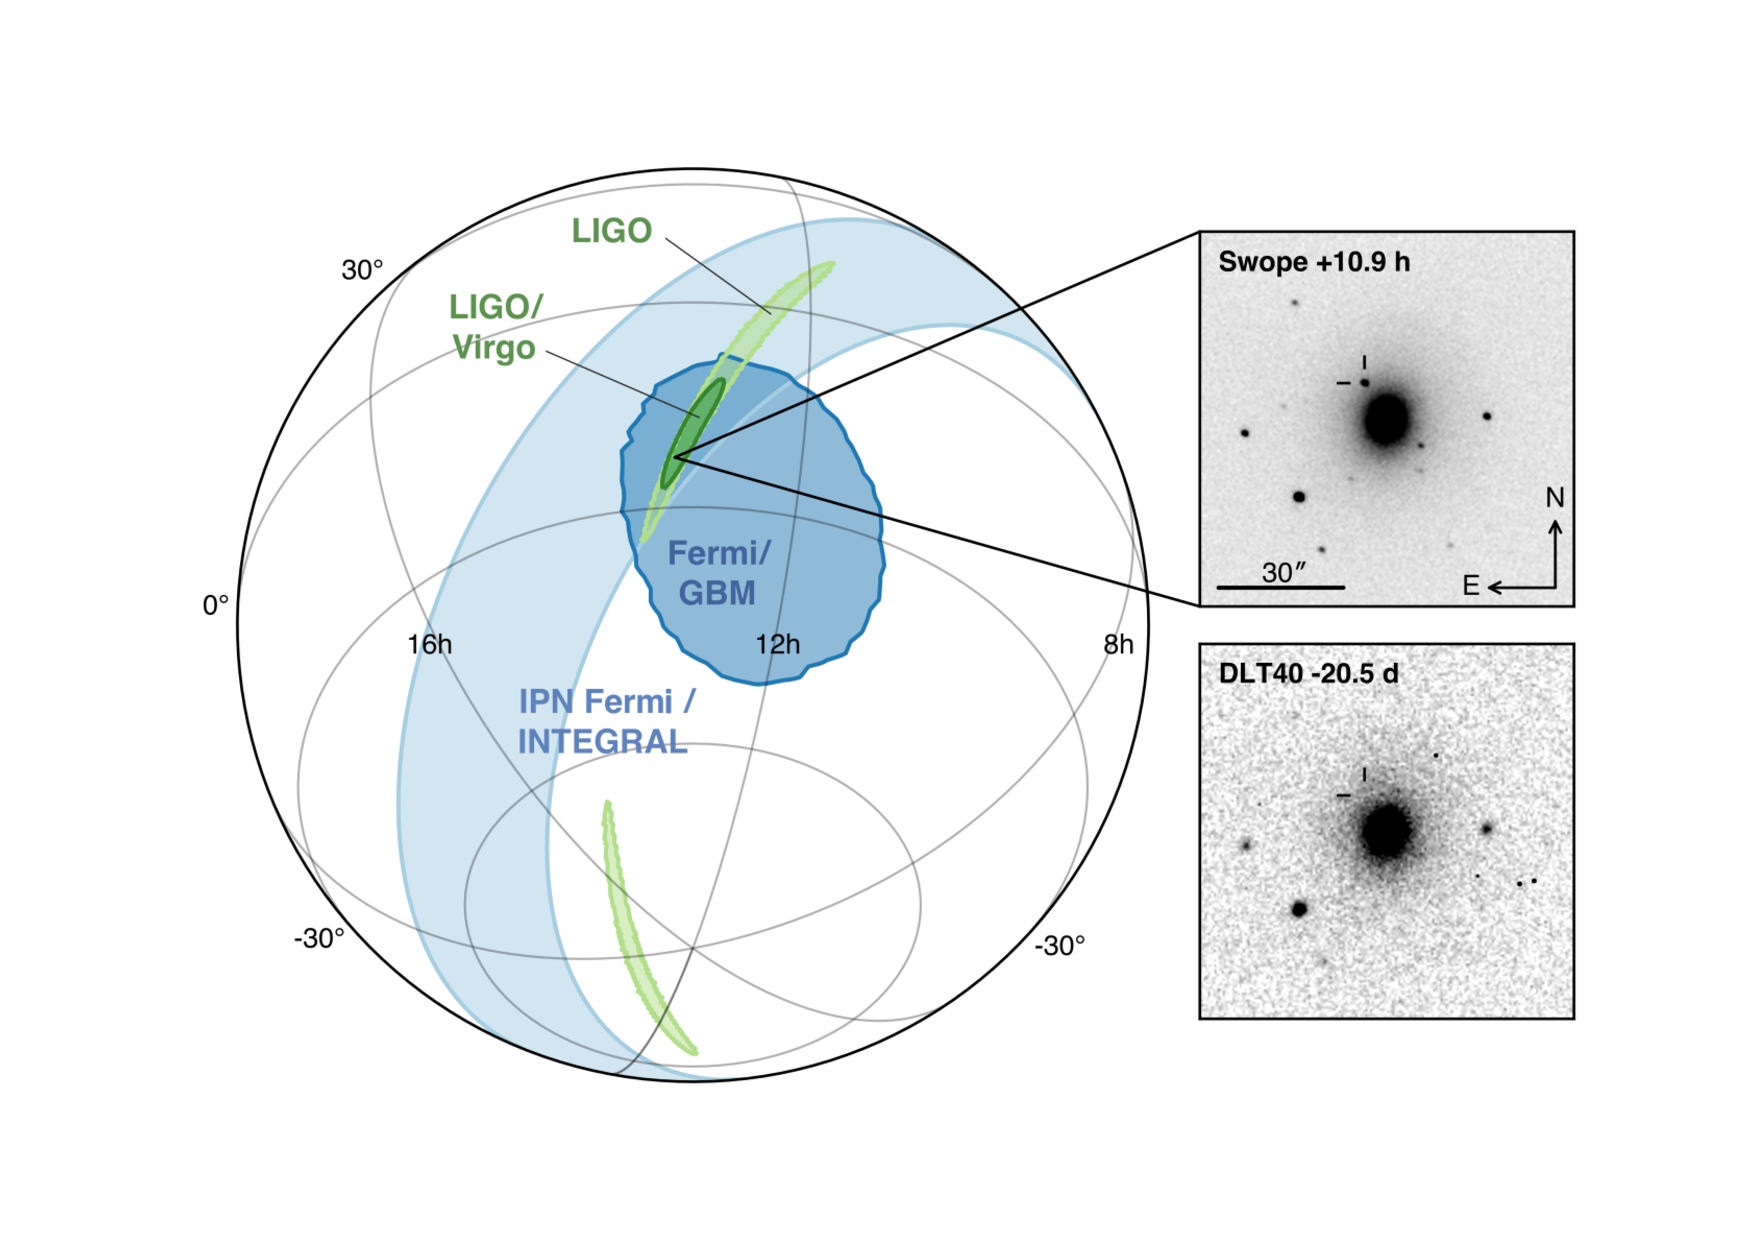
\includegraphics[width=\columnwidth]{GW170817_MMA_Skymap} 
\captionof{figure}{Lokaliseringen af kilonovaen baseret på ankomsttidspunktet af tyngebølge-signal til de forskellige detektorer, samt GBM lokalisationen. Figuren er taget fra \cite{abbottb}\label{fig1}}
\end{figure}





\section{Baggrund}\label{bag}

For at forstå, hvorfor dette fænomen var søgt efter med sådan en ihærdighed, samt hvorfra navnet kilonova stammer, kræver det en del baggrundsviden. 

Den kemiske sammensætning af universet er på ethvert tidspunkt et produkt af startbetingelserne og de processer, der undervejs virker for at drive den kemiske berigelse. I begyndelsen af vores observerbare univers var Big Bang. Big Bang efterlader et univers primært bestående af hydrogen og helium. Tyngdekraften får ur-gassen til at blive til fragmenter i mindre og mindre stykker, som til sidst danner galakserne og deres bestanddele - stjerner. Under tilpas høj tæthed og temperatur (der bliver opnået inde i centrum af alle stjerner) undergår hydrogen og helium kernefusioner. Kernefusion er den proces, hvorved to atomkerner fusionerer. To hydrogen-kerner støder sammen og laver helium, tre helium-kerner støder sammen og laver karbon, en karbonkerne og en heliumkerne støder sammen og laver ilt, o.s.v. ... På denne måde bliver grundstofferne tungere og tungere. Denne proces kan lade sige gøre, fordi bindingsenergien af tungere grundstoffer er højere end for lettere grundstoffer. Der kan derfor vindes energi ved at omdanne lette grundstoffer til tunge. Denne fusions-proces er energikilden til alle tændte stjerner i universet. 


De højeste bindingsenergier findes i grundstofferne jern ($\mathrm{Fe}_{26}^{56}$) og nikkel ($\mathrm{Ni}_{28}^{58}$) med atomtal på hhv. 26 og 28 og massetal på hhv. 56 og 58. Atomtallet betyder, at de hver indeholder hhv. 26 og 28 protoner, og massetallene betyder, at de hver indeholder hhv. 56 og 58 protoner og neutroner. Fordi jern og nikkel har de højeste bindingsenergier, er det også de tungeste grundstoffer, der naturligt laves ved fusion. Tungere grundstoffer end jern og nikkel er allesammen lavet på basis af neutronindfangning. Neutronindfangning betyder, at en atomkerne optager en fri neutron. Dette kan ske, fordi neutronen er ladningsløs, og der ikke er nogen elektrostatisk frastødning mellem atomkernen og den frie neutron. Ved en neutronindfangning stiger massetallet for et grundstof med 1, fordi der er kommet en ekstra neutron i kernen. Hvis en jernkerne og en fri neutron støder sammen, vil det hedde $\mathrm{Fe}_{26}^{56} + \mathrm{n} \rightarrow \mathrm{Fe}_{26}^{57} + \gamma$, hvor n er neutronen, og $\gamma$ er en foton. $\mathrm{Fe}_{26}^{57}$ er en stabil isotop af jern, men hvis nu der bliver ved at blive indfanget neutroner, vil det til sidst kunne hedde $\mathrm{Fe}_{26}^{58} + \mathrm{n} \rightarrow \mathrm{Fe}_{26}^{59} + \gamma$. $\mathrm{Fe}_{26}^{59}$ er \textit{ikke} en stabil isotop og vil beta-henfalde til cobalt plus en neutrino ( $\mathrm{Fe}_{26}^{59} \rightarrow  \mathrm{Co}_{27}^{59} + \nu_e$), hvorved atomtallet stiger med 1. Betahenfald er den proces, hvor en neutron henfalder til en proton og en neutrino.


\section{$r$-processen}\label{rproc}

\begin{figure}
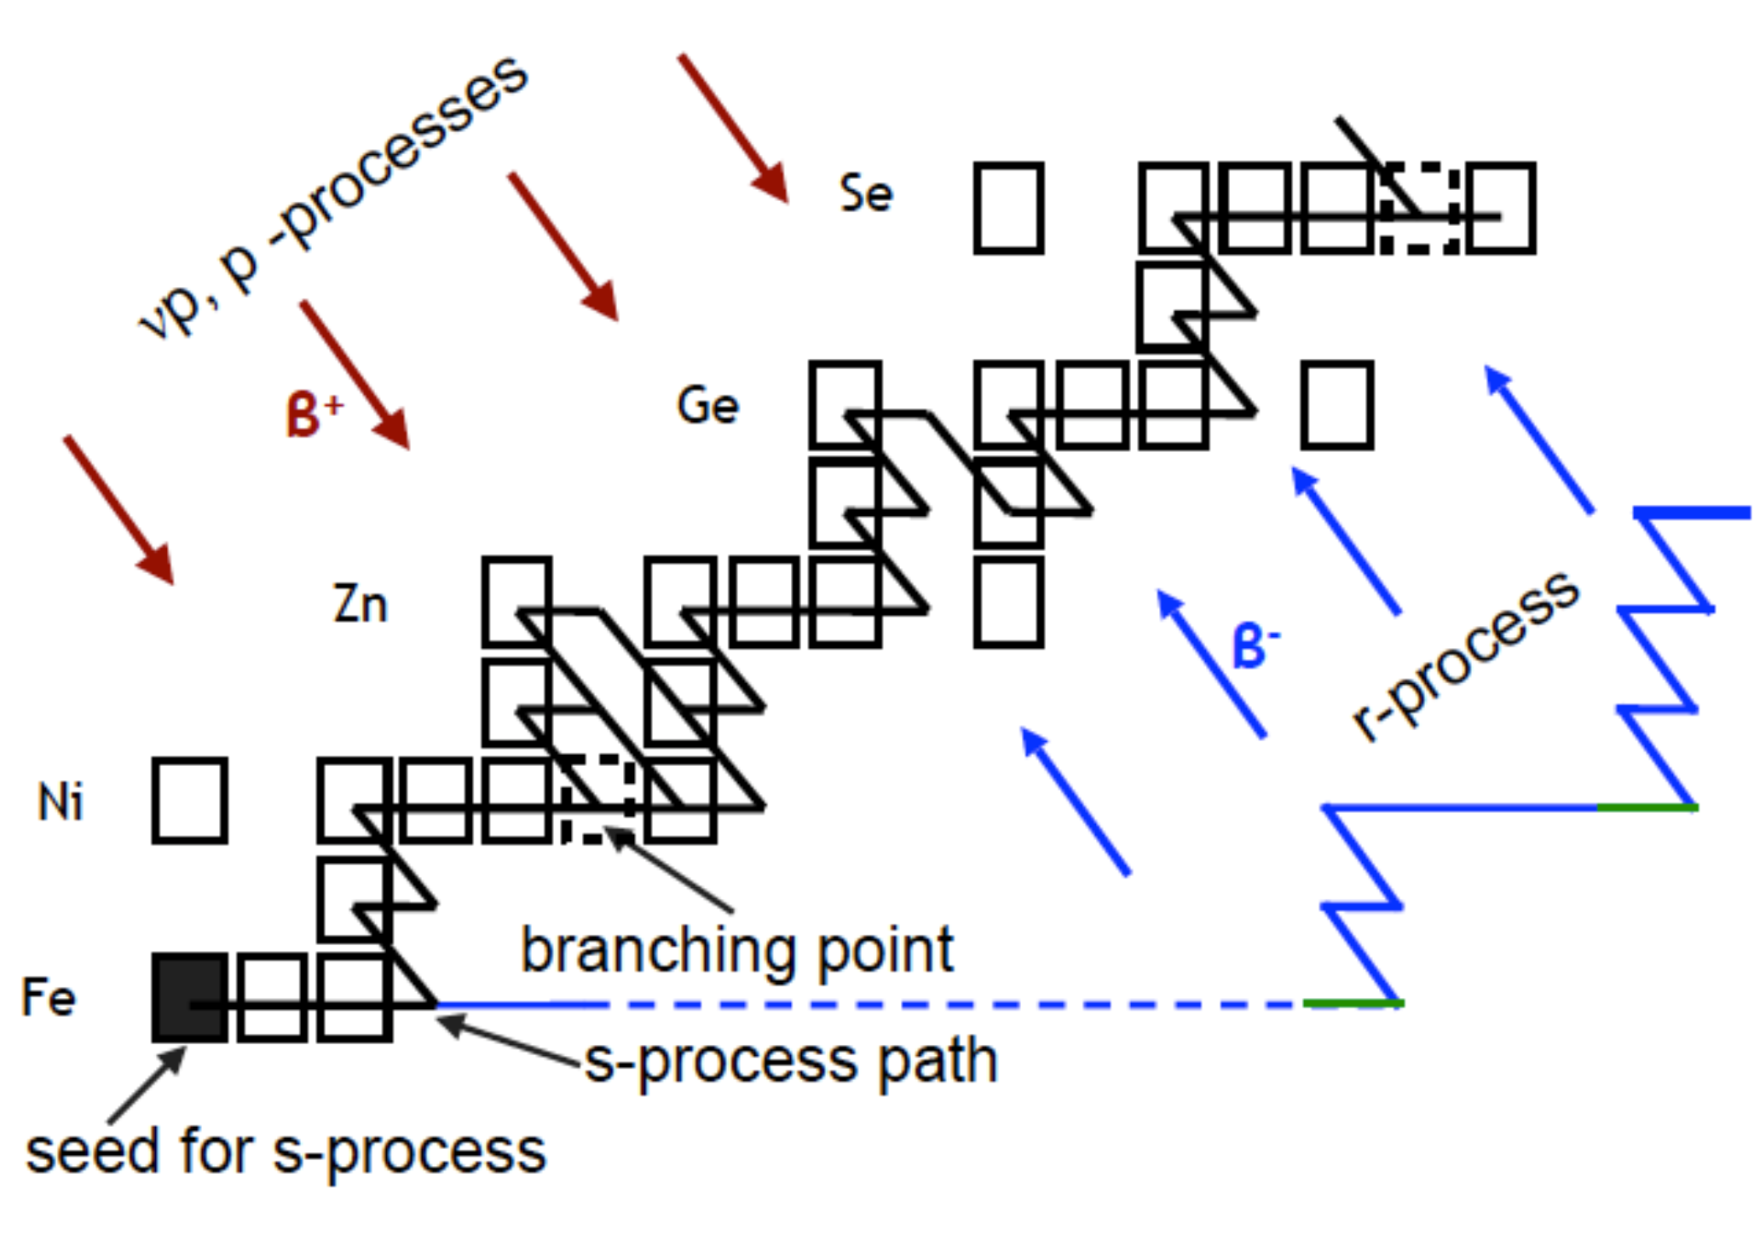
\includegraphics[width=\columnwidth]{r-process2.pdf}
\captionof{figure}{Illustration af $s$- og $r$ processen. $S$-processen er den sorte streg, der følger de stabile isotoper. Steder, hvor der er huller i isotop-stigen, gør, at $s$-processen skal bruge lang tid til at kravle opad i atomtal. $R$-processen, derimod, kan meget hurtigt berige kim-grundstoffer til de tungeste grundstoffer i vores periodiske system.}
\end{figure}

Neutronindfangnings-processen opdeles i to klasser, som bliver separeret på baggrund af neutronindfangningsraten - altså hastigheden, hvormed neutroner bliver fanget - i forhold til beta-henfalds raten. $s$-processen, hvor $s$ står for slow, betyder at neutronindfangningsraten er langsommere end beta-henfaldet. I $s$-processen vil enhver neutronindfangning til en ustabil isotop være efterfulgt at et beta-henfald til et grundstof med én proton mere, og derfor højere i det periodiske system. $S$-processen kan i princippet give alle de tungere grundstoffer op til polonium ($\mathrm{Po}_{210}^{84}$), men er for langsom til at kunne berige vores univers i tilstrækkelig grad og hurtigt nok. $r$-processen ($r$ står for rapid), derimod, er den hurtigste proces, hvor neutroner bliver indfanget hurtigere end det nye element kan nå at beta-henfalde. Denne proces kan virke på meget korte tidsskalaer og har i princippet ikke nogen øvre grænse for, hvor tunge grundstoffer den kan lave. Problemet med $r$-processen er, at den kræver en enorm tæthed af frie neutroner - en tæthed, der i praksis er meget svær at opnå. Der er dog ét sted i universet, hvor neutrontætheden er enorm. Neutronstjerner. Neutronstjerner er restproduktet af en stor del af de supernovaer, der har hydrogen i deres spektre (type II), og er kompakte objekter, der ikke er større end ca. 10 km i diameter. Neutronstjerner vejer som regel omkring 1.4 gange så meget som vores sol og består sandsynligvis i høj grad af neutroner. De har en tynd ydre skal af jern. Grunden til deres store andel af neutroner er, at tyngdekraften er så høj, at de elektroner og protoner, der måtte være, er blevet presset sammen til neutroner. Hvis man på én eller anden måde kan få en neutronstjerne revet fra hinanden, ville det kunne give den tilstrækkelige tæthed af frie neutroner til at drive $r$-processen.

\section{Neutronstjerne-sammenstød}\label{ns}

\begin{figure}
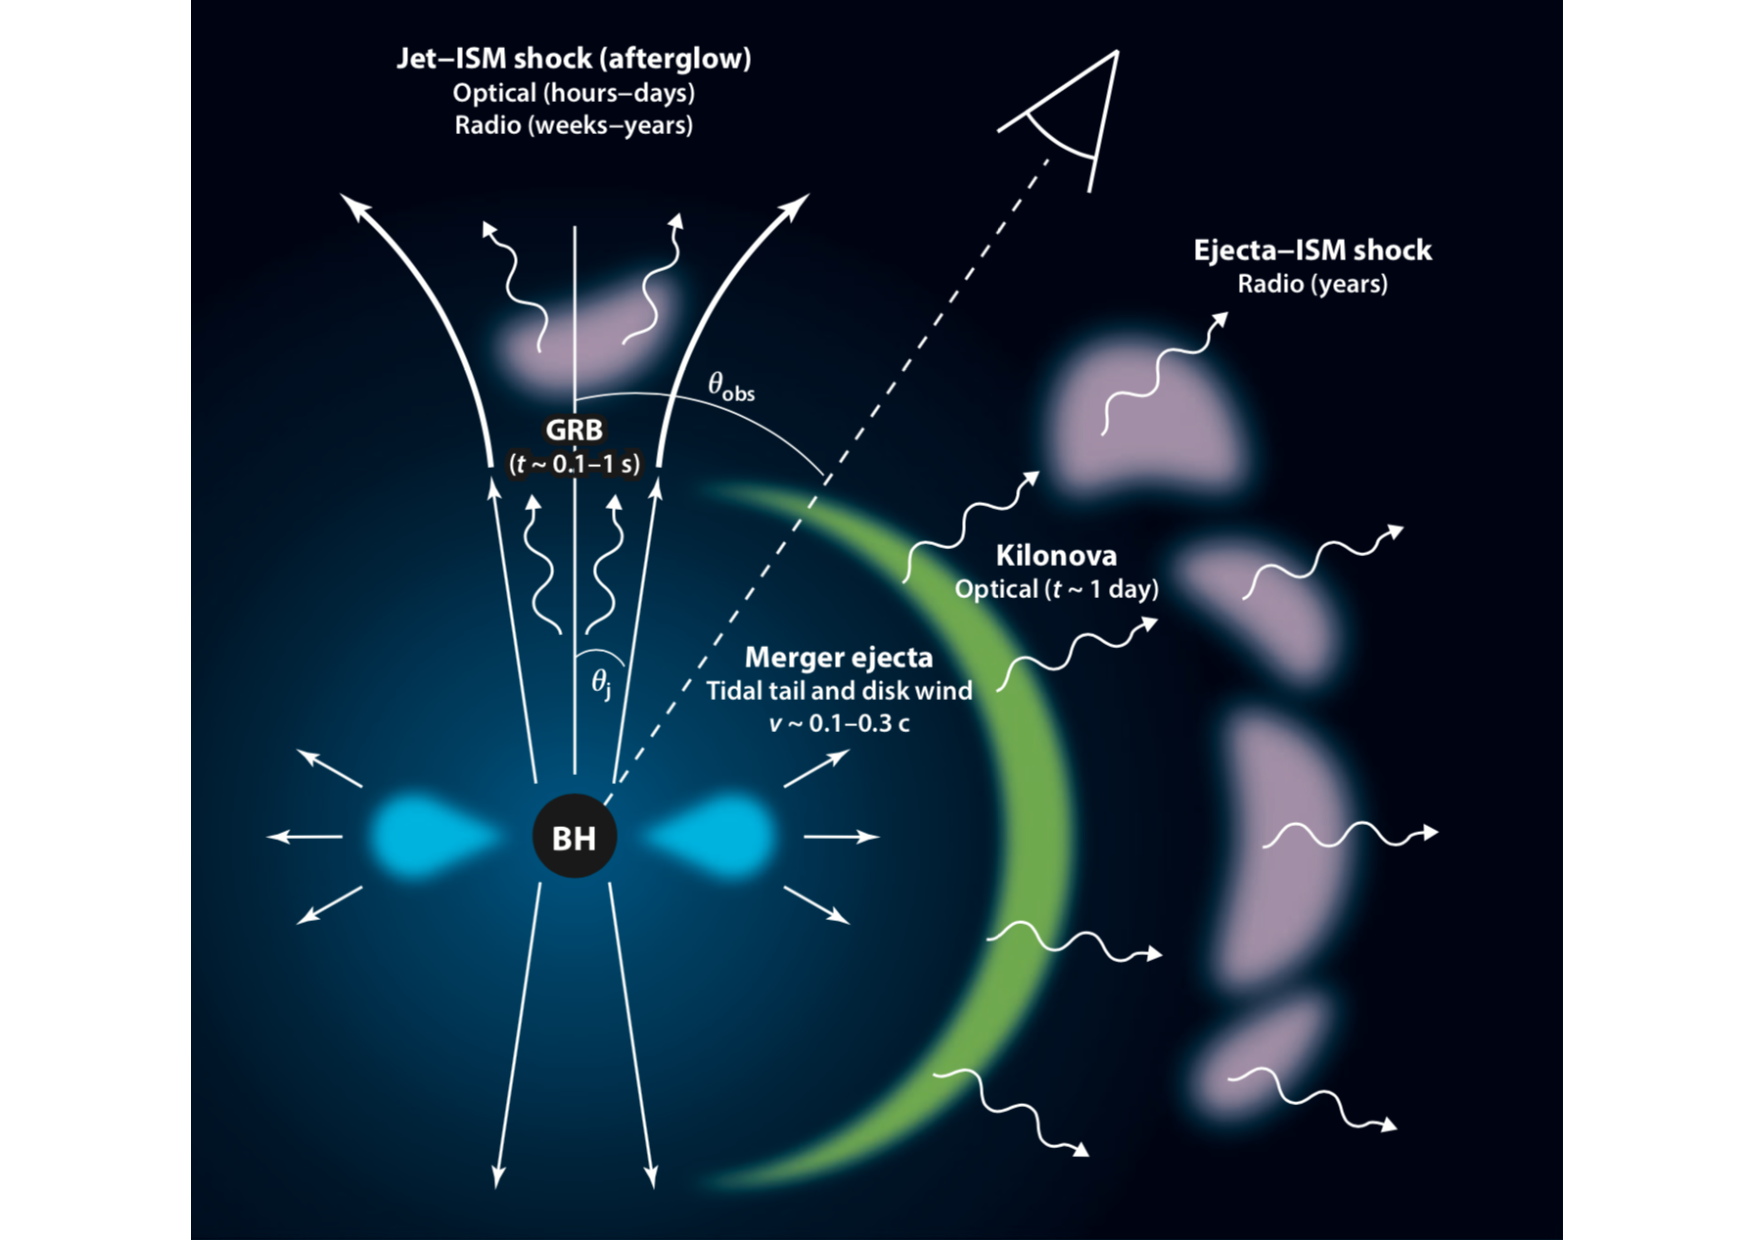
\includegraphics[width=\columnwidth]{KN_scematic_berger.pdf}
\captionof{figure}{Skematisk oversigt over, hvordan vi forestiller os, kilonovaen bliver dannet. Centralt er det nydannede sorte hul (BH), hvor de to blå "dråber" repræsenterer de to neutronstjerner, der er ved at smelte sammen. Figuren er fra \cite{berger}}
\end{figure}

I 1974 blev det første binære neutronstjerne-system fundet, kaldet Hulse-Taylor-systemet, opkaldt efter dets opdagere. Her fandt man det første bevis for tilstedeværelsen af tyngdestråling fra henfaldet af omløbsbanen af dette system. %(Mellem opdagelsen af kilonovaen og offentliggørelsen, blev Rainer Weiss, Barry C. Barish og Kip S. Thorne tildelt Nobelprisen i fysik for opdagelsen af tyngdebølger.) 
Henfaldet af omløbsbanen af de to neutronstjerner betyder, at de langsomt bevæger sig nærmere og nærmere hinanden under udsendelse af tyngdebølger, hvilket er i overensstemmelse med Einsteins generelle relativitetsteori. De to neutronstjerner i Hulse-Taylor-systemet vil støde sammen om ca. 300 millioner år.  

Sammenstødet mellem to neutronstjerner har, fordi det er det optimale sted for $r$-processen, været fokus for en del teoretiske undersøgelser. De modeller, der er udviklet for sammenstødet, viser enstemmigt, at en væsentlig del af den totale masse vil blive slynget ud i rummet i det plan, som neutronstjernerne roterer om hinanden. Grunden til dette er, at som omløbsbanen henfalder, vil rotationshastigheden af systemet stige. På et tidspunkt, ca. samtidig som de to neutronstjerner støder sammen, vil rotationshastigheden af de yderste dele af neutronstjernerne være hurtigere end undvigelseshastigheden for en binært neutronstjernesystem. Derfor vil de blive slynget ud. Den store mængde, nu frie, neutroner vil med det samme blive absorberet af jern-laget og drive $r$-processen hele vejen til de tungeste grundstoffer. De nydannede, meget tunge grundstoffer vil så beta-henfalde og radioaktivt spalte sig under udsendelse af en meget stor mænge lys. De teoretiske modeller forudsiger, at den totale mængde lys, der bliver udsendt, vil være ca. 1000 gange så stor som den mængde lys, der bliver udsendt ved en normal nova. Deraf navnet kilonova. Tusind gange så lysstærk som en nova. Det friske $r$-proces-syntetiserede materiale vil indeholde alle de tungeste grundstoffer i det periodiske system - inklusive guld, sølv, og platin.

Neutronstjerne-sammenstød har yderlige to fysiske signaturer, som var yderst eftersøgte. Hidtil havde man ikke nogle troværdige målinger af, hvilke systemer der giver anledning til korte gammaglimt. Med den samtidige detektion at et kort gammaglimt og tyngdebølger fra binært system, der vejer ca. lige så meget som to neutronstjerner, og en kilonova, var der endegyldigt bevis for, at i hvert fald nogle korte gammaglimt bliver lavet af neutronstjerne-sammenstød. Den anden signatur er den, at "lydstyrken" af tyngdebølger er bestemt af perioden af bølgen. Fra rødforskydningen af værtsgalaksen og denne periode kan vi ret præcist måle en absolut afstand - en måling, der er meget svær at lave, og som har stor betydning for vores estimater af universets alder og udvidelseshistorie. Denne måling er konsistent med målinger, som kommer fra f.eks PLANCK-teleskopet. Ved at måle flere af disse afstande håber vi på at kunne finde afvigelser mellem PLANCK-målingerne og tyngdebølgerne, der vil åbne døren til nye modeller for vores univers. 


\section{Observationer}\label{obs}

\begin{figure}
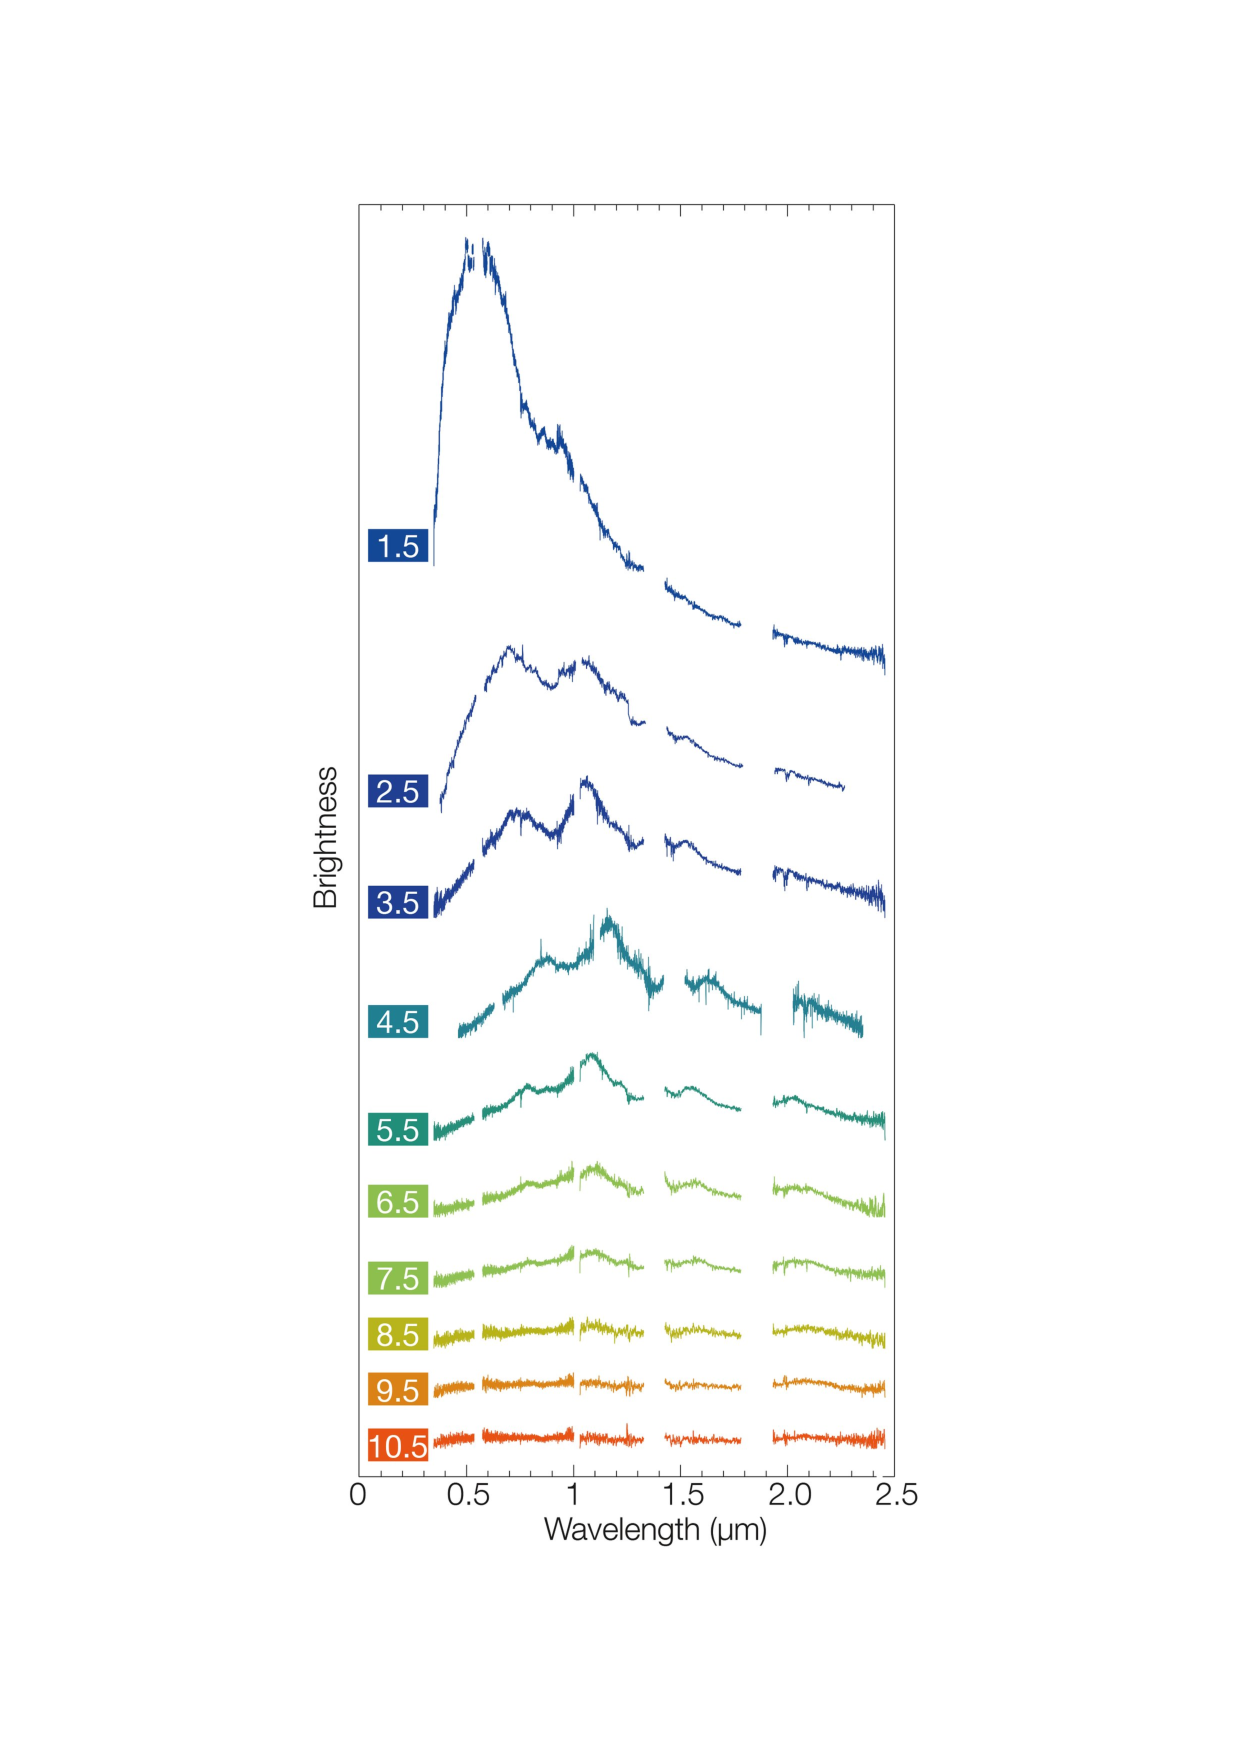
\includegraphics[width=\columnwidth]{specs.pdf}
\captionof{figure}{Spektre af kilonovaen AT2017gfo. Hvis man sammenligner spektrene med de teoretiske spektre i figur \ref{kasen}, kan man se, at den kvalitative overensstemmelse er stor. Alle spektrene har brede signaturer og en udvikling, hvor lyset med de korte bølgelængder forsvinder relativt til de længere. Hvad vi også kan se er, at der stadig er betydelige forskelle mellem de teoretiske og de observerede spektre. Spektrene her er præsenteret i \cite{pian} og \cite{smartt}. \label{spec}}
\end{figure}


Fordi neutronstjerne-sammenstødet var forbundet med stor forventning, var det højt prioriteret på teleskoper verden over. Derfor findes der et væld af observationer på tværs af hele det elektromagnetiske spektrum fra røntgenstråling til radio. Observationerne bekræfter dele af de teoretiske forestillinger om, hvordan sådan et fænomen måtte se ud, hvor især det optiske lys afslører, hvordan de tungeste grundstoffer bliver dannet. De mest detaljerede informationer fås fra et sæt spektroskopiske observationer taget med VLT-instrumentet X-shooter i Chile. De er vist i fig. \ref{spec}. Spektrene udsender en stor del af deres lys i den ultraviolette del af spektret til at starte med, men som dagene går, bliver en større del af lyset udsendt ved længere bølgelængder. Dette er lige netop det tegn, vi ville forvente at se, hvis materialet, der udsender lyset, hovedsageligt består af $r$-proces-grundstofferne. Det er svært at identificere signaturer fra individuelle grundstoffer i spektrene, modsat hvad der er muligt i spektre af supernovaer. Grunden til dette er, at vi ikke har tilstrækkelig viden om overgangene i de grundstoffer, som udsender lyset, samt at udbredelseshastigheden af det lysende materiale nærmer sig 30 procent af lysets hastighed. Den enorme hastighed gør, at alle individuelle signaturer bliver spredt ud i bølgelængder på grund af hhv. rød- og blåforskydninger af lyset. Den store udbredelseshastighed af det lysende materiale stemmer godt overens med modellerne, hvor de to neutronstjerner drejer rundt om hinanden med tæt ved lysets hastighed, kort før de brager sammen. 


\section{Teoretiske modeller}\label{teo}


\begin{figure}
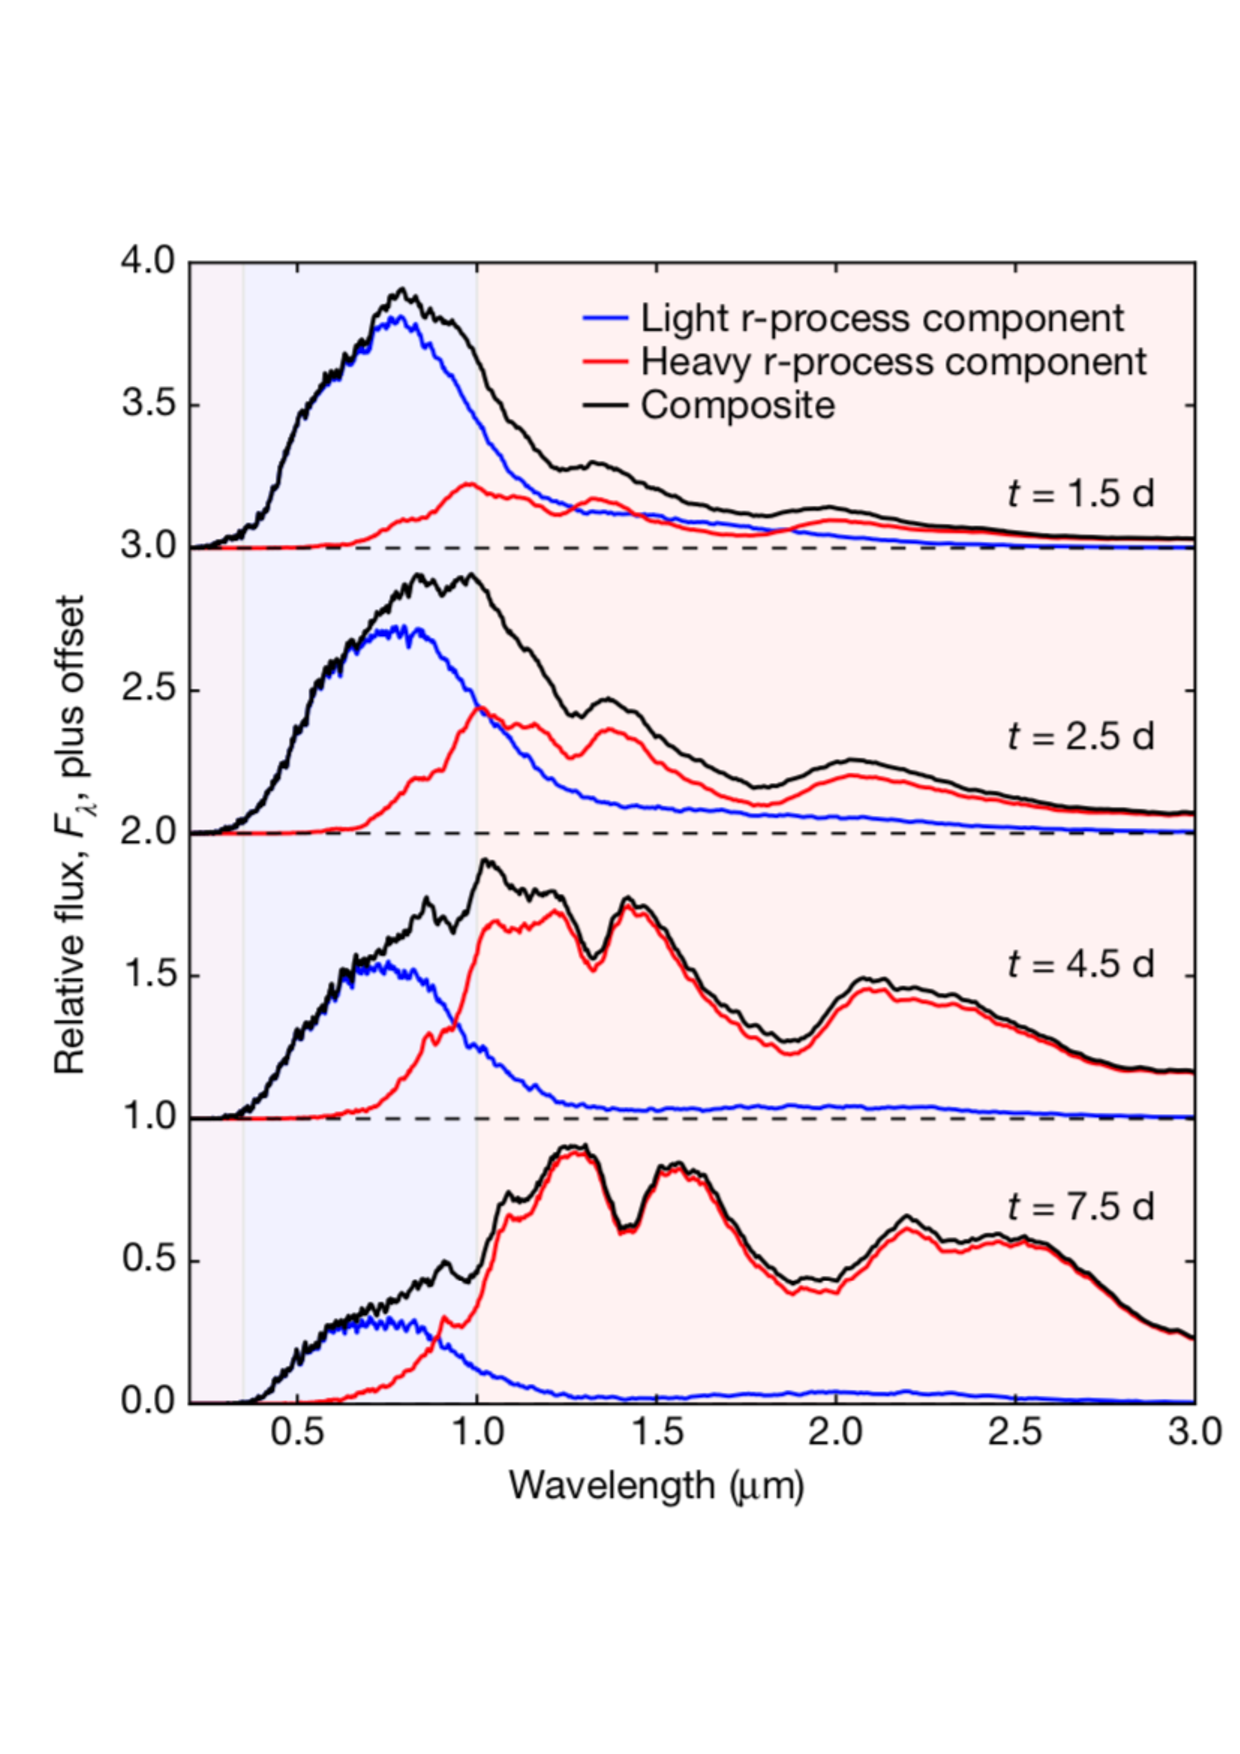
\includegraphics[width=\columnwidth]{kasen_kn}
\captionof{figure}{Syntetiske spektre af en kilonova. De forskellige paneler viser tidsudviklingen, hvor man kan se, at en større del af lyset blev udsendt ved længere bølgelængder i de senere tider. Dette er, fordi de tungeste grundstoffer forholdsvis absorberer det blå lys. Denne figur er fra \cite{kasen}  \label{kasen}}
\end{figure}

Inden den første kilonova var fundet, var der allerede udviklet detaljerede modeller for, hvordan de kunne se ud. Baseret på vores viden om atomfysik og  simuleringer af sammenstødet mellem de to neutronstjerner var det muligt at forsøge at forudsige, hvordan lyset fra en kilonova vil se ud. Det er det, der er vist i fig. \ref{kasen}. Her har man taget en mængde neutronstjernemateriale og ladet det henfalde ifølge lovene for kernefald. Disse simuleringer tillader, at vi for ethvert tidpunkt kan finde grundstof-sammensætningen og på baggrund af denne forsøge at forudsige, hvordan lyset fra en sådan sammensætning vil se ud. Ens for en kombination af de tunge grundstoffer er, at de absorberer forholdsvis mere af lyset med kortere bølgelængder. Det lys, der ikke kan slippe ud ved de kortere bølgelænger, slipper så ud ved længere bølgelængder, og kilonovaen vil derfor fremstå mere rød. Den store mængde blandede, radioaktive stoffer fra alle de tungeste grundstoffer i det periodiske system gør desuden, at lysstyrken skal falde på en meget karakteristisk måde - noget, vi ser reproduceret i dataen fra kilonovaen. Som man kan se ved at sammenligne de teoretiske spektre i fig. \ref{kasen} med de observerede spektre i fig. \ref{spec} er der både ligheder og forskelligheder. Den overordnede struktur ser nogenlunde ens ud med spektre domineret af brede signaturer, der udviser en udvikling fra lys domineret af kortere bølgelængder til længere bølgelængder. Positionerne af de enkelte signaturer og deres relative størrelse er imidlertid ikke forudsagt korrekt. Dette skyldes primært, at de tungeste grundstoffer stadig er relativt uudforsket land, hvor antallet af overgange og deres styrker stadig er ukendte. Dette skyldes primært, at udforskningen af dette er en meget dyr og besværlig affære.



\section{Konklusioner}
Denne detektion af tyngdebøgler sammen med en kilonova er så betydningsfuld, fordi der med ét er blevet ført bevis for adskillige store, ubesvarede spørgsmål. Denne opdagelse har bidraget til forståelsen af, hvad oprindelsen til disse korte gammaglimt er, hvor de fleste af de tungeste grundstoffer bliver dannet. Samtidig har det givet en helt uafhængig, nøjagtig måling af Hubble-konstanten. Dette betyder, at det guld, du har i dine tænder, på dine hænder, om din hals eller i din computer er blevet syntetiseret på et eller andet tidspunkt før Jorden blev skabt i et sammenstød mellem to neutronstjerner. 


\begin{thebibliography}{9}
\bibitem[1]{abbotta} \emph{GW170817: Observation of Gravitational Waves from a Binary Neutron Star Inspiral.},
Abbott, B. P., et al., Physical Review Letters 119, 161101 (2017).

\bibitem[2]{abbottb} \emph{Multi-messenger Observations of a Binary Neutron Star Merger.},
Abbott, B. P., et al., The Astrophysical Journal Letters, 848:L12 (2017).

\bibitem[3]{lattimer} \emph{Black-hole-neutron-star collisions.},
Lattimer, J. M. \& Schramm, D. N., The Astrophysical Journal Letters 192:L145 (1974).

\bibitem[4]{berger} \emph{Short-Duration Gamma-Ray Bursts.},
Berger, E., Annu. Rev. Astron. Astrophys. 52:43–105 (2014).

\bibitem[5]{kasen} \emph{Origin of the heavy elements in binary neutron-star
mergers from a gravitational-wave event.},
Kasen, D, et al., Nature, Volume 551, Issue 7678, pp. 80-84 (2017)

\bibitem[6]{pian} \emph{Spectroscopic identification of r-process nucleosynthesis in a double neutron-star merger.},
Pian, E, et al., Nature, Volume 551, Issue 7678, pp. 67–70 (2017)

\bibitem[7]{smartt} \emph{A kilonova as the electromagnetic counterpart to a gravitational-wave source.},
Smartt, S. J., et al., Nature, Volume 551, Issue 7678, pp. 75–79 (2017)









\end{thebibliography}

\captionsetup[figure]{labelformat=empty}

\begin{figure}[!htbp]
\begin{center}
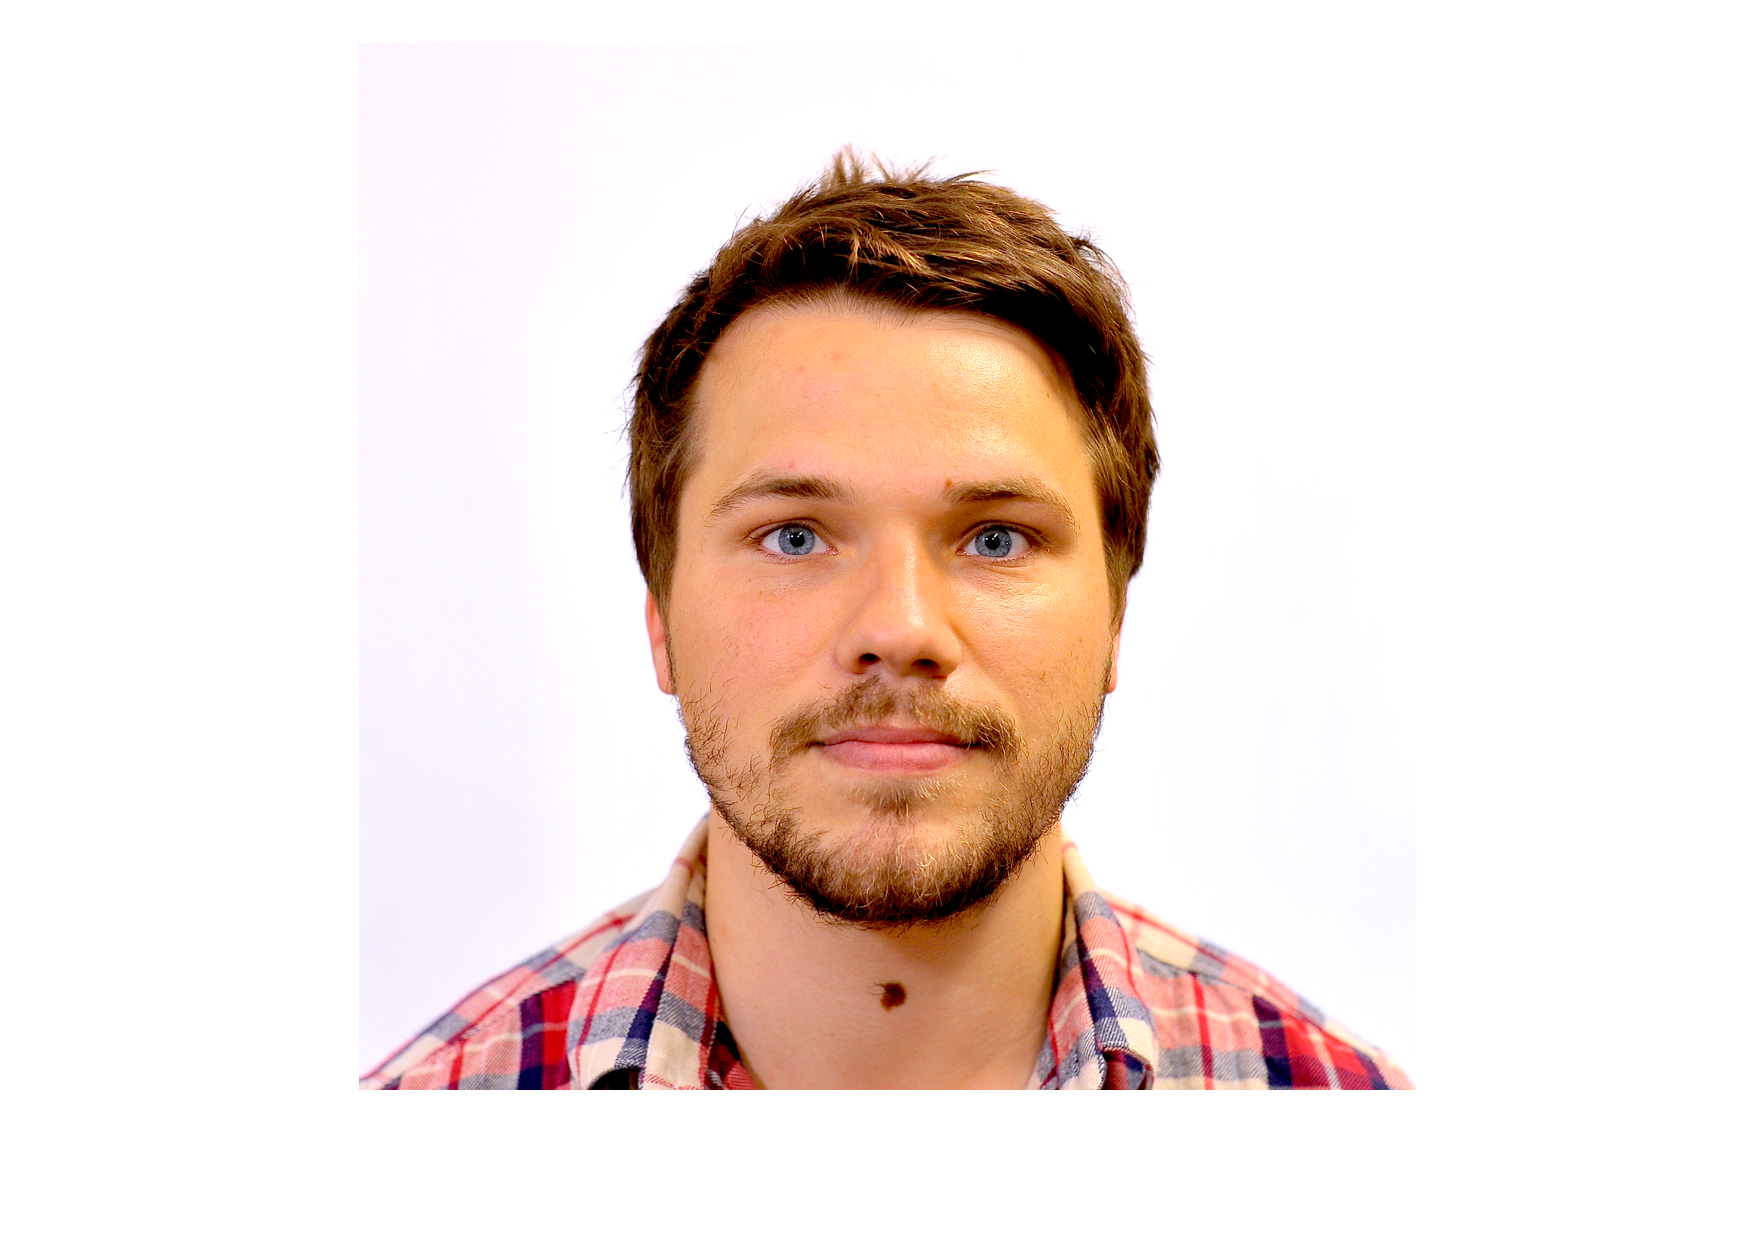
\includegraphics[width=0.5 \columnwidth]{me}
\captionof{figure}{Jonatan Selsing er postdoktoral forsker på The Cosmic Dawn Center, Niels Bohr Instituttet, Københavns Universitet, og forsker i optiske modstykker til tyngdebølger.}
\end{center}
\end{figure}


\end{document}
